\documentclass[11pt,a4paper]{article}
\usepackage[margin=22mm]{geometry}
\usepackage{graphicx,booktabs,amsmath,longtable}
\usepackage[hidelinks]{hyperref}
\setlength{\parindent}{0pt}\setlength{\parskip}{6pt}\emergencystretch=3em
\newcommand{\uv}{\ensuremath{\mu\mathrm{V}}}
\title{FORCe window boundaries and filtering in movement-locked EEG\\[3pt]\large A matched two-participant pilot research note}
\author{Satyam Awasthi}\date{}
\begin{document}\maketitle
\begin{abstract}
Independent one-second FORCe calls can introduce discontinuities when reconstructed windows are joined. We evaluate those boundaries and an offline adaptation: continuous high-pass filtering, one-second cleaning, and low-pass filtering of a three-second segment before cropping. Four processing conditions compare bandpass filtering with and without FORCe, and split filtering with and without FORCe. Across 2,562 matched trials, the +0.5~s Cz median jump was 3.778~\uv\ with bandpass-first FORCe and 0.440~\uv\ with split filtering, versus 0.416~\uv\ in the bandpass no-FORCe control and 0.414~\uv\ in the split no-FORCe control. In the no-FORCe control, applying the low-pass to three-second segments instead of continuously changed the retained signal by less than $10^{-9}$~\uv. Broader FORCe-related waveform differences nevertheless remained. This pilot is descriptive; lower boundary steps or changed ERP waveforms do not establish preservation of underlying neural signals or better artifact removal.
\end{abstract}
\section{Questions and scope}
\textbf{Q1: Does FORCe introduce abnormal changes at window joins?} Compare cleaned outputs with their filtering-matched no-FORCe controls, assessing jumps relative to ordinary sample changes and the common reference voltage range, and checking whether per-window centring contributes to signal-level shifts.

\textbf{Q2: How effectively does the proposed design attenuate joining discontinuities, and what effects remain after cropping?} Assess actual pre/post-low-pass jumps, the spread of known injected disturbances, finite-segment versus continuous low-pass filtering, and broader ERP amplitude/timing changes. This tests the purpose of the proposed design without assuming that smoothing resolves a discontinuity. FORCe is optional; practical consequences are evaluated rather than a benefit assumed.
FORCe combines wavelets, independent-component analysis and thresholding \cite{daly}. Empirically calibrated settings are retained. The supplied Graz study discusses error-related EEG responses approximately 0.4--0.8~s after movement onset \cite{graz}; the proposed join at +0.5~s intersects that interval.
\section{Methods}
\subsection{Data and four processing conditions}
Both pilot participants (mle01 and spe30), all eligible task recordings, and pre/post/retest sessions are included. Eight-channel EEG is sampled at 500~Hz; Cz and FCz are primary. Movement-locked extraction is $[-1.5,1.5)$~s. The three cleaning windows are $[-1.5,-0.5)$, $[-0.5,0.5)$ and $[0.5,1.5)$~s: movement onset is no longer a join. This three-second extraction is a deliberate comparison adaptation, not a reproduction of the default two-second integration associated with the supplied study \cite{graz}. The historical integration joins two independently cleaned one-second halves at onset. Here both FORCe conditions use identical shifted boundaries to avoid confounding their filtering comparison with boundary placement.
Continuous filters are applied separately to valid recording segments. Acquisition-loss markers (event code 255), nonfinite samples and timestamp gaps create recording-segment boundaries. The complete three-second interval must lie outside two-second guards at each segment endpoint. This guard is part of trial eligibility: valid events, a complete three-second interval, and no acquisition gaps or filter-guard overlap are required. The guard is an existing conservative policy, not a proven settling bound.
Butterworth filters have order four and are applied forward/backward. The upper cutoff remains 20~Hz. The historical bandpass and separate high-/low-pass designs differ, so this evaluates practical pipelines rather than filter order alone.
\begin{center}\small\begin{tabular}{cll}\toprule
ID & Continuous filtering & Three-second processing \\
\midrule
1 & 1--20 Hz bandpass & No FORCe \\
2 & 1--20 Hz bandpass & Three 1 s FORCe calls \\
3 & 1 Hz high-pass & No FORCe; 20 Hz low-pass \\
4 & 1 Hz high-pass & Three 1 s FORCe calls; 20 Hz low-pass \\
\bottomrule\end{tabular}\end{center}

The two FORCe conditions (2 and 4) and their matching no-FORCe controls (1 and 3), listed in the table above, are cropped to $[-1,1)$~s, baseline-corrected over $[-0.2,0)$~s, and rejected if absolute amplitude exceeds 100~\uv. FORCe failures reject the complete trial. The supplied FORCe implementation flags channels exceeding +200~\uv\ for channel estimation. Our integration instead rejects the trial when this occurs, avoiding the channel-estimation code path. This positive-only check is distinct from the final absolute-amplitude rejection. Source decomposition depth remains two, and no additional thresholds or library behaviour are changed for this comparison.
Condition 1 is the bandpass no-FORCe reference; condition 2 is bandpass-first FORCe; condition 4 is FORCe with split filtering; condition 3 is the matching split-filter no-FORCe control. Split/rejoin without cleaning is checked for exact sample preservation. Condition 4 is saved before and after low-pass filtering. Main comparisons use trials accepted in all four conditions; separate retention counts document excluded trials.
\subsection{Boundary measurements}
The jump $J$ is the absolute voltage change across the adjacent samples straddling a boundary. For trial $i$, channel $c$, and boundary time $b$,
\[
J_{icb}=|x_{ic}(b)-x_{ic}(b-2~\mathrm{ms})|.
\]
The same measurement at onset ($b=0$) supplies a non-join location. Ordinary changes are absolute adjacent-sample differences away from the inspected boundaries and onset. A fixed 100~ms interval ($\pm50$~ms) around each of $-0.5$, 0 and $+0.5$~s is excluded to reduce contamination of the reference distribution by local discontinuities. This exclusion does not establish that all filtering effects are confined to 100~ms. Each jump's empirical percentile and the fraction at or above the 99th percentile describe rarity, not an artifact label or formal significance. Percentiles are condition-specific; low-pass filtering changes the reference distribution.
Let $S_{ic}$ denote the robust voltage range of trial $i$ on channel $c$. Define it from the bandpass no-FORCe reference (condition 1), so each condition uses the same trial/channel denominator rather than its own altered waveform range:
\[
S_{ic}=Q_{95}(x^{(1)}_{ic})-Q_{5}(x^{(1)}_{ic}),\qquad J^*_{icb}=J_{icb}/S_{ic}.
\]
This imposes no Gaussian assumption. A degenerate scale is a zero or nearly zero voltage range, which makes division undefined or unstable; such normalised measurements are not interpreted. The matched data pass the analysis check $S>10^{-10}$~\uv. Cz and FCz are primary because these central/frontocentral channels are selected for the ERP comparison. Maximum jumps across all eight channels are supporting summary statistics; waveform plots show actual individual trials.
\subsection{Filtering-only and FORCe-related waveform residuals}
A residual is the point-by-point difference between two specified processing outputs, not necessarily an error. The comparisons below separate short-segment filtering from cleaning-related changes.
\begin{enumerate}
\item \textbf{Finite-segment filtering:} condition 3 minus continuous high-pass followed by continuous low-pass, after identical crop and baseline. The additional continuous reference uses the same sequential high-pass and low-pass coefficients as conditions 3/4. Condition 1 instead uses a single continuous bandpass design. Thus this comparison isolates finite-segment low-pass application, while comparison with condition 1 evaluates the broader design change.
\item \textbf{Injected boundary:} a unit persistent step or a one-sample spike is injected at each join into an otherwise unchanged no-FORCe sequence. This test uses condition 4's final low-pass coefficients to assess how that proposed design handles abrupt joining disturbances. Its control is the same input without injection; subtracting the two outputs isolates the response to the known disturbance. It does not run FORCe or replay condition 1. By linearity, subtracting injected/uninjected outputs equals filtering the disturbance. Normalisation is by injected amplitude. Short- and long-segment responses use the actual low-pass coefficients and endpoint handling. Synthetic plots are before baseline correction to isolate filtering; real-trial residuals include baseline correction.
\item \textbf{Actual cleaning:} condition 4 minus 3, and condition 2 minus 1. Both include intended artifact removal and potentially unwanted changes; neither estimates neural error.
\end{enumerate}
For recorded EEG trials, the normalised difference between waveforms $A$ and $B$ at time $t$ is $r_{ic}(t)=[x_{A,ic}(t)-x_{B,ic}(t)]/S_{ic}$. Median, 95th percentile and maximum absolute residual are measured in the full epoch, its outer 200~ms at each end, the 0.2--0.9~s response interval, and $\pm50$~ms at both joins. Values are reported in \uv\ and reference-range fractions. No arbitrary cutoff declares a boundary resolved.
\paragraph{Centring and reconstruction audit.} A centring audit uses the first three eligible trials per recording, with continuously 1~Hz-high-pass-filtered input, as used by condition 4. The existing wavelet/SOBI path is reconstructed without rejection or coefficient thresholding. Mean shifts and nonconstant RMS residuals distinguish level changes from broader reconstruction differences; the supplied implementation is not edited.
\paragraph{Condition-difference waveforms.} For each participant/session and channel, displaced-minus-non-displaced averages use identical trials. Peak times identify the largest absolute deflection within 0.2--0.9~s. Differences between conditions may reflect selection of different peaks, rather than a latency change in the same ERP component. The 0.2--0.9~s interval is the pilot's broad descriptive search interval, encompassing the approximately 0.4--0.8~s response interval in the supplied study; it is not a separately validated component window.
\subsection{Statistical interpretation}
Two-participant results are descriptive. Adjacent voltage samples within a trial are temporally dependent; they must not be treated as independent observations in a t-test. Many trials from two participants likewise do not provide population-level participant replication. No population-level significance or equivalence claim is made. Filtering may spread abrupt changes \cite{widmann}; cropping the padded three-second segment to two seconds removes its outer context, but leaves the joins at $-0.5$ and $+0.5$~s inside the analysis interval.
\section{Results}\subsection{FORCe boundary discontinuities}
There are 29 recordings, 2,915 trial rows, 2,799 eligible complete intervals, and 2,562 trials accepted by all four conditions. Eligible means that the complete three-second interval passes event, acquisition-gap and filter-guard checks. Accepted additionally means passing cleaning and final-amplitude checks. Common is the four-way intersection used for all waveform comparisons. This intersection may exclude the most contaminated trials, so separate retention counts remain important.
\begin{center}\small\begin{tabular}{lrrrrrr}\toprule
Participant & Eligible & 1 & 2 & 3 & 4 & Common \\
\midrule
mle01 & 1411 & 1179 & 1201 & 1182 & 1203 & 1176 \\
spe30 & 1388 & 1386 & 1387 & 1386 & 1387 & 1386 \\
Pooled & 2799 & 2565 & 2588 & 2568 & 2590 & 2562 \\
\bottomrule\end{tabular}\end{center}
\subsubsection{Magnitude and rarity}
Pooled matched-trial statistics are shown below. $J/S$ is the median of per-trial normalised jumps, not a ratio of separately pooled medians. $J/S$ is expressed as a percentage. The Q99-exceedance percentage is the percentage of trials whose jump at the specified boundary equals or exceeds that trial's 99th-percentile ordinary adjacent-sample change. It is not the percentage of all samples exceeding their own percentile threshold. Participant-specific summaries appear in the appendix. Pooled percentages weight participants by retained trial counts.
\begin{center}\small\begin{tabular}{lcrrrrr}\toprule
Ch. & Join & ID & Median (\uv) & $J/S$ (\%) & $Q_{95}$ (\uv) & \shortstack{Trials $\geq Q_{99}$\\(\%)} \\
\midrule
Cz & -0.5 & 1 & 0.330 & 1.27 & 1.190 & 0.6 \\
Cz & -0.5 & 2 & 1.550 & 5.82 & 8.976 & 42.3 \\
Cz & -0.5 & 4 & 0.306 & 1.20 & 1.035 & 1.4 \\
Cz & -0.5 & 3 & 0.327 & 1.25 & 1.182 & 0.6 \\
Cz & +0.5 & 1 & 0.416 & 1.57 & 1.459 & 2.1 \\
Cz & +0.5 & 2 & 3.778 & 14.17 & 16.329 & 66.9 \\
Cz & +0.5 & 4 & 0.440 & 1.72 & 1.445 & 5.8 \\
Cz & +0.5 & 3 & 0.414 & 1.56 & 1.452 & 2.2 \\
FCz & -0.5 & 1 & 0.335 & 1.22 & 1.217 & 0.7 \\
FCz & -0.5 & 2 & 1.689 & 6.08 & 10.294 & 43.7 \\
FCz & -0.5 & 4 & 0.312 & 1.13 & 1.053 & 1.4 \\
FCz & -0.5 & 3 & 0.334 & 1.20 & 1.200 & 0.7 \\
FCz & +0.5 & 1 & 0.426 & 1.53 & 1.597 & 2.2 \\
FCz & +0.5 & 2 & 4.205 & 15.14 & 18.369 & 68.7 \\
FCz & +0.5 & 4 & 0.473 & 1.70 & 1.554 & 6.8 \\
FCz & +0.5 & 3 & 0.423 & 1.53 & 1.589 & 2.2 \\
\bottomrule\end{tabular}\end{center}
At +0.5~s in Cz, median jumps are 3.778~\uv\ for bandpass-first FORCe and 0.440~\uv\ for split FORCe; the split control is 0.414~\uv. Rarity fractions are 66.9\% and 5.8\% respectively. These are pooled pilot descriptions.
Figure~\ref{fig:boundary} shows the cumulative distributions: a rightward shift means larger normalised jumps. These are distributions across matched trials, not paired differences.
\begin{figure}[htbp]\centering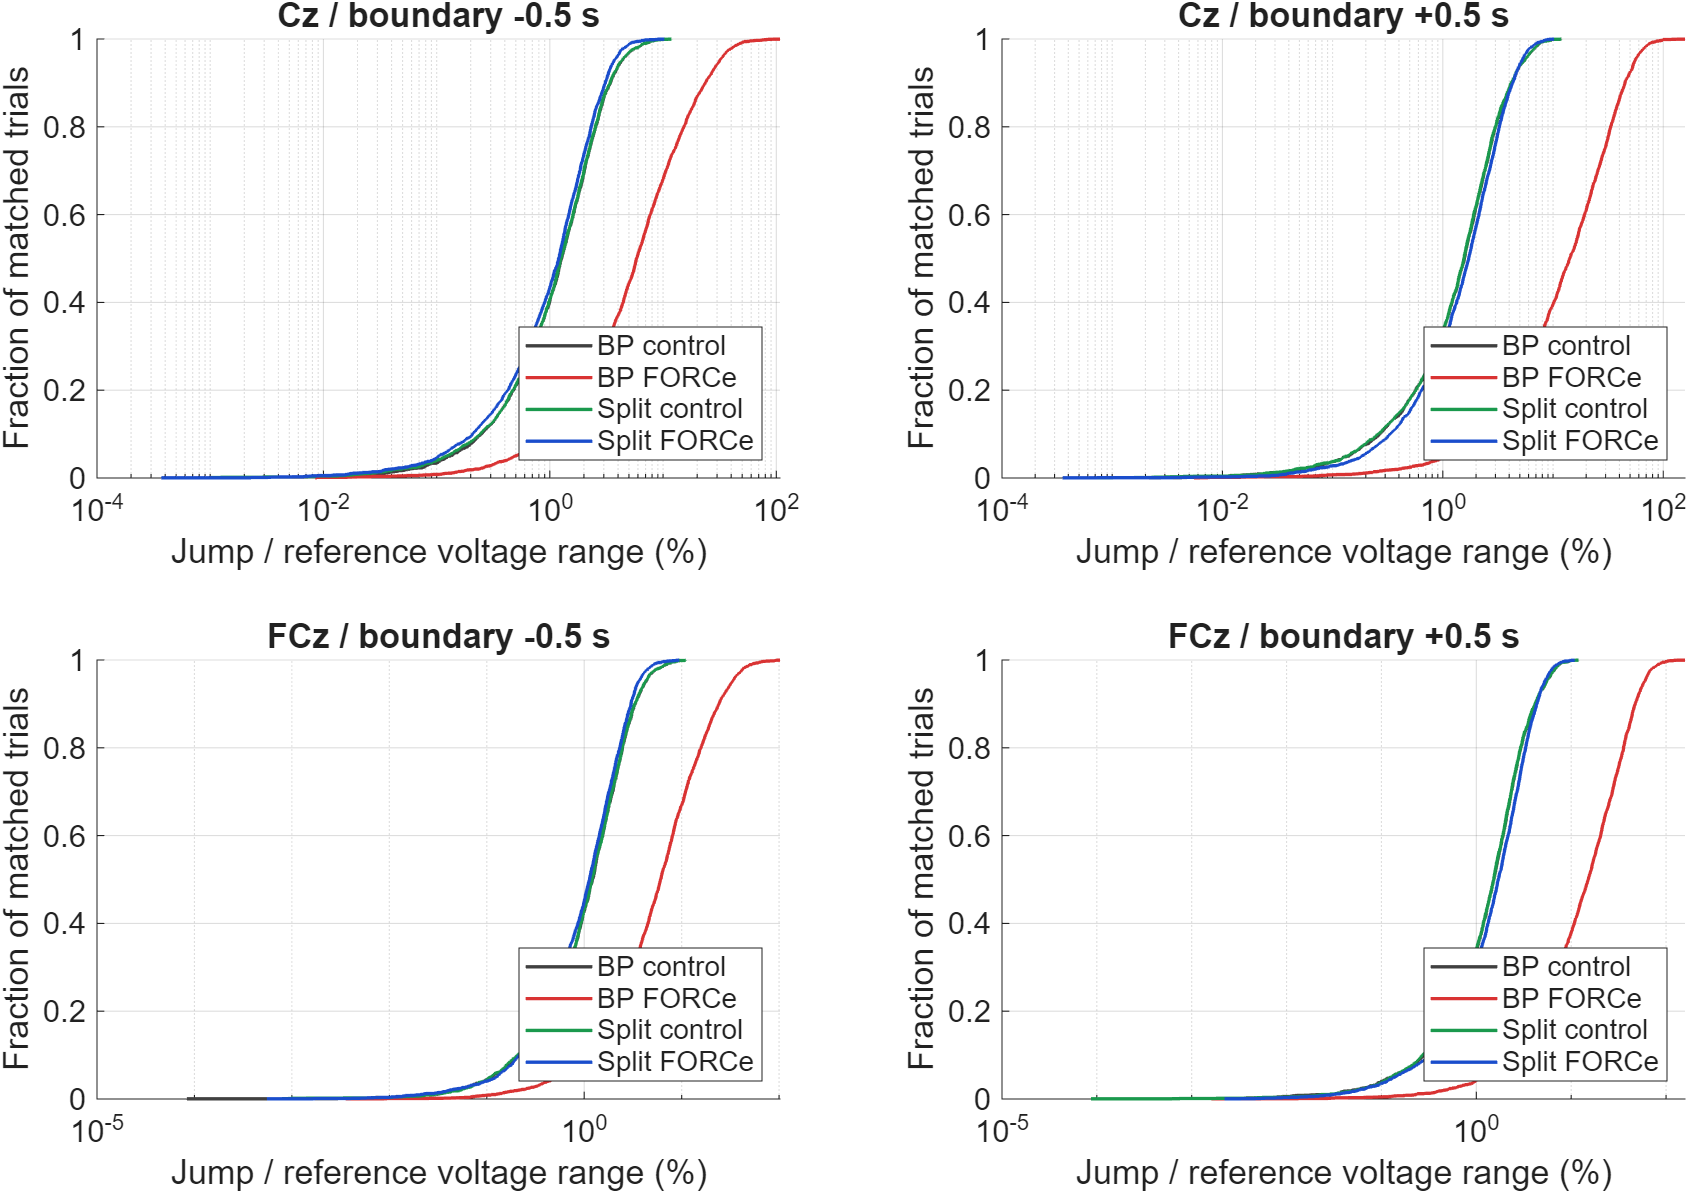
\includegraphics[width=\linewidth]{figures/boundary_distributions.png}
\caption{\label{fig:boundary}Matched-trial distributions of normalised jumps in Cz and FCz; BP denotes bandpass. The denominator is fixed across conditions. Onset and all-eight-channel results are supporting measurements.}\end{figure}
\clearpage\subsubsection{Paired boundary effects}
Contrast A: condition 2 minus 1 (original FORCe effect). B: condition 4 minus 3 (proposed FORCe effect). C: condition 2 minus 4 (change in FORCe usage). A positive value means a larger jump in the first condition. These are medians of paired trial differences, not differences between marginal medians. The final column reports the percentage of matched trials whose boundary jump is larger in the first condition than in the second condition of the contrast; it does not use Q99. These paired comparisons quantify cleaning-related boundary effects, including possible signal-level shifts; the reconstruction audit examines one potential contribution. For example, 91.5\% for contrast A at +0.5~s in Cz means bandpass-first FORCe exceeds its no-FORCe control in 91.5\% of matched trials. Normalised paired changes retain the same condition-1 trial/channel scale $S$.
\begin{center}\small\begin{tabular}{lclrrr}\toprule
Ch. & Join & Contrast & Median $\Delta J$ (\uv) & $\Delta J/S$ (\%) & \shortstack{Larger jump\\(\%)} \\
\midrule
Cz & -0.5 & A & 1.099 & 4.25 & 85.1 \\
Cz & -0.5 & B & -0.027 & -0.12 & 42.8 \\
Cz & -0.5 & C & 1.156 & 4.48 & 87.0 \\
Cz & +0.5 & A & 3.215 & 12.37 & 91.5 \\
Cz & +0.5 & B & 0.015 & 0.06 & 51.7 \\
Cz & +0.5 & C & 3.281 & 12.44 & 91.4 \\
FCz & -0.5 & A & 1.285 & 4.51 & 85.6 \\
FCz & -0.5 & B & -0.026 & -0.10 & 43.8 \\
FCz & -0.5 & C & 1.307 & 4.76 & 87.9 \\
FCz & +0.5 & A & 3.693 & 13.14 & 91.5 \\
FCz & +0.5 & B & 0.020 & 0.07 & 52.5 \\
FCz & +0.5 & C & 3.683 & 13.13 & 92.1 \\
\bottomrule\end{tabular}\end{center}

\clearpage\subsubsection{Proposed output before and after low-pass}
\begin{center}\small\begin{tabular}{lcrrrrrr}\toprule
Ch. & Join & Median pre & Median post & $Q_{95}$ pre & $Q_{95}$ post & Max pre & Max post \\
\midrule
Cz & -0.5 & 4.814 & 0.306 & 15.188 & 1.035 & 36.212 & 2.350 \\
Cz & +0.5 & 6.511 & 0.440 & 20.112 & 1.445 & 39.980 & 2.787 \\
FCz & -0.5 & 4.699 & 0.312 & 15.234 & 1.053 & 42.828 & 2.667 \\
FCz & +0.5 & 6.805 & 0.473 & 21.413 & 1.554 & 47.801 & 2.973 \\
\bottomrule\end{tabular}\end{center}
This table compares condition 4 immediately before and after its final 20~Hz low-pass. Each row summarises the adjacent samples straddling the specified boundary, $b-2$~ms and $b$, across the same matched trials. Maxima are across trials at that boundary, not searched over time. All values are in \uv. Each maximum can arise from a different trial. The reduction demonstrates attenuation of adjacent-sample changes; it does not establish removal of broader effects.
\subsubsection{Representative individual trials}
Two examples are selected at the median and 95th-percentile rank of condition 2's Cz normalised jump at +0.5~s. Every overlay uses the same trial and channel. This selection illustrates representative and upper-tail behaviour in bandpass-first FORCe; it is not an average treatment effect.
\begin{figure}[htbp]\centering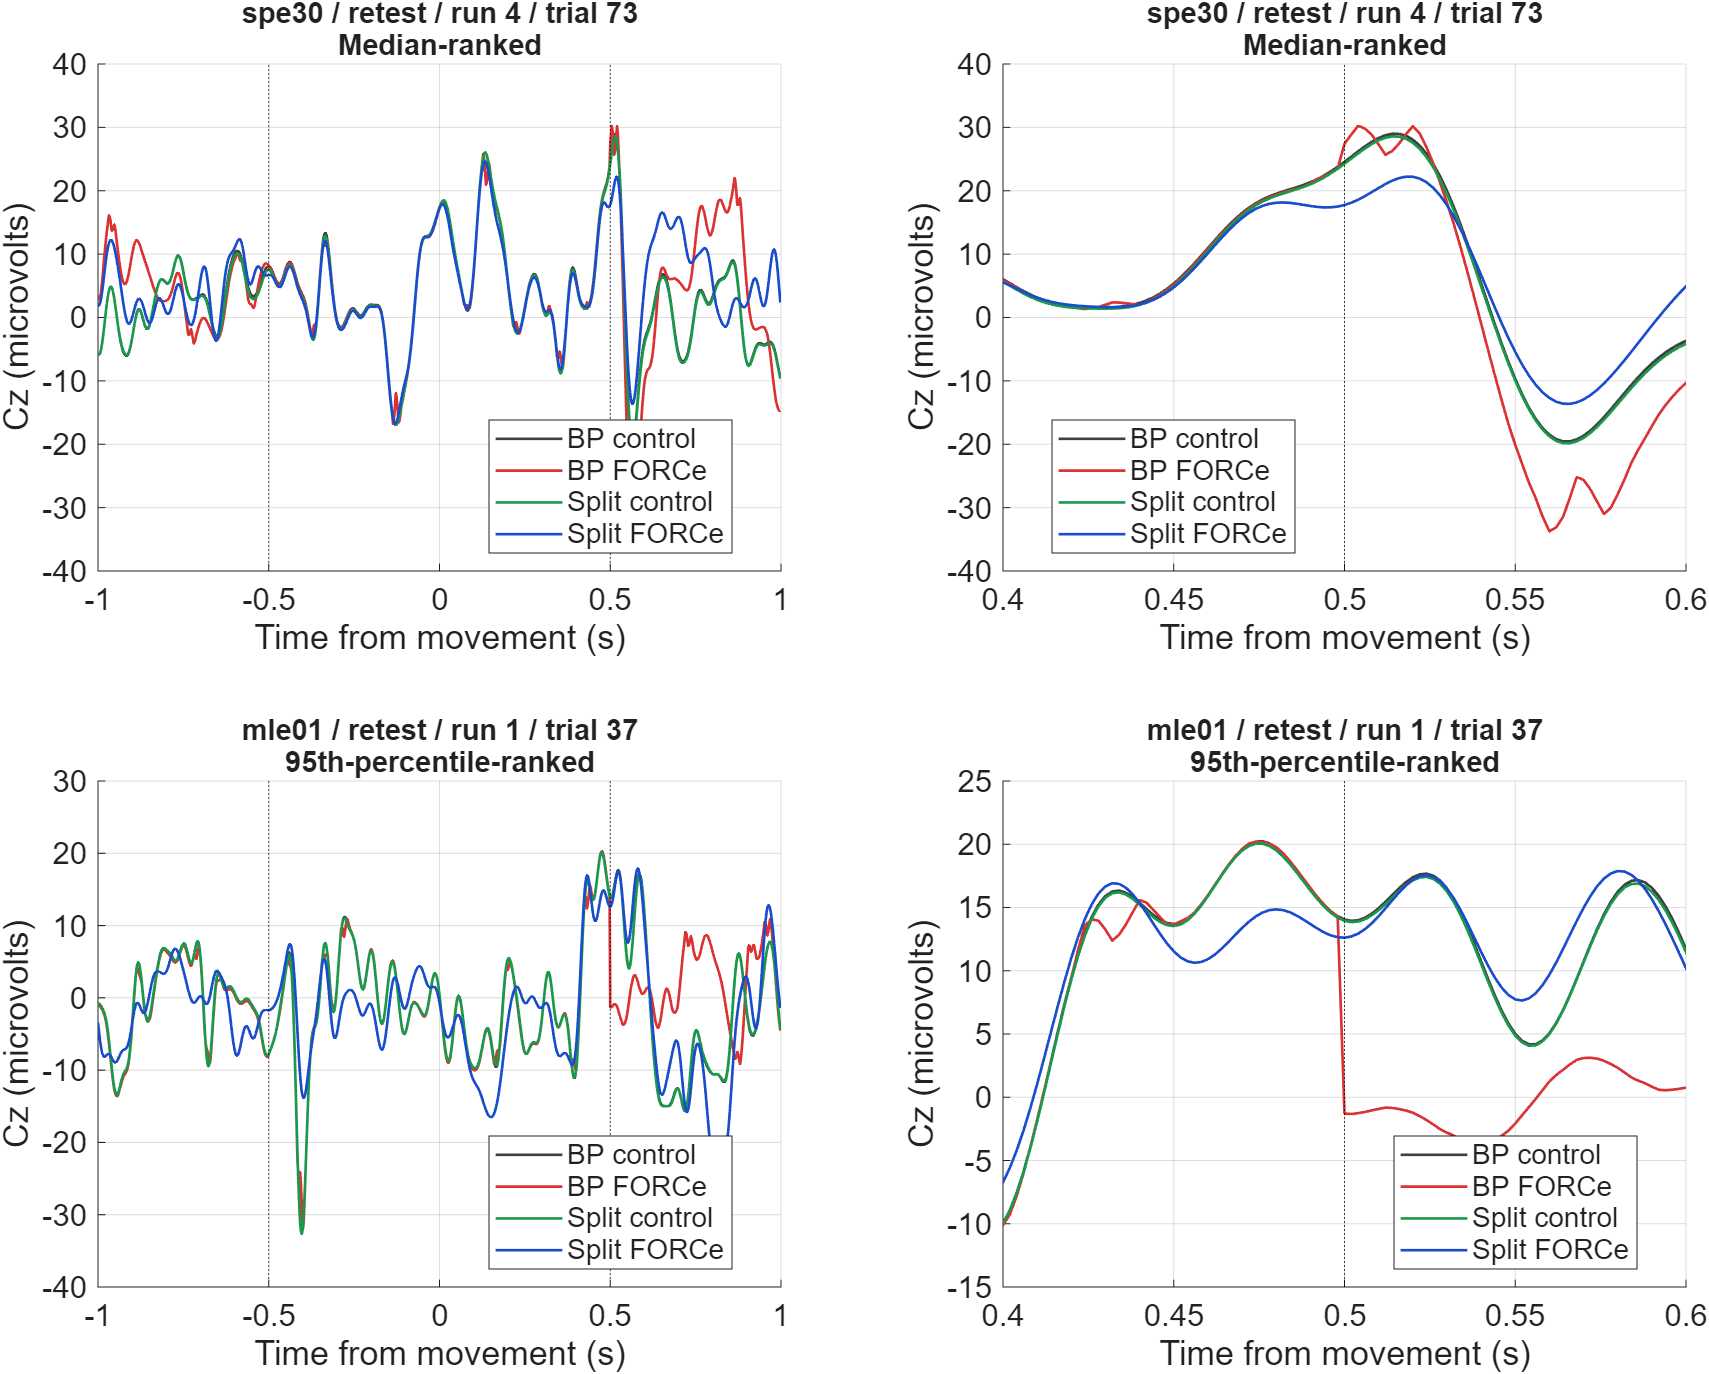
\includegraphics[width=\linewidth]{figures/representative_trials.png}
\caption{Full-epoch and join-detail overlays for representative trials. A smoother trace alone cannot establish preservation of the underlying EEG.}\end{figure}
\clearpage\subsection{Filtering effects and broader waveform changes}\subsubsection{Finite-segment filtering effects}
Finite-segment low-pass filtering produced negligible differences from continuous low-pass filtering in the tested no-FORCe data. The largest finite-segment filtering residual in the matched Cz/FCz data is $6.28\times10^{-10}$~\uv\ anywhere in the retained epoch. This bounds the tested no-FORCe inputs, extraction length and filter only. It does not directly establish the same endpoint-effect bound for FORCe-cleaned segments.
\begin{figure}[htbp]\centering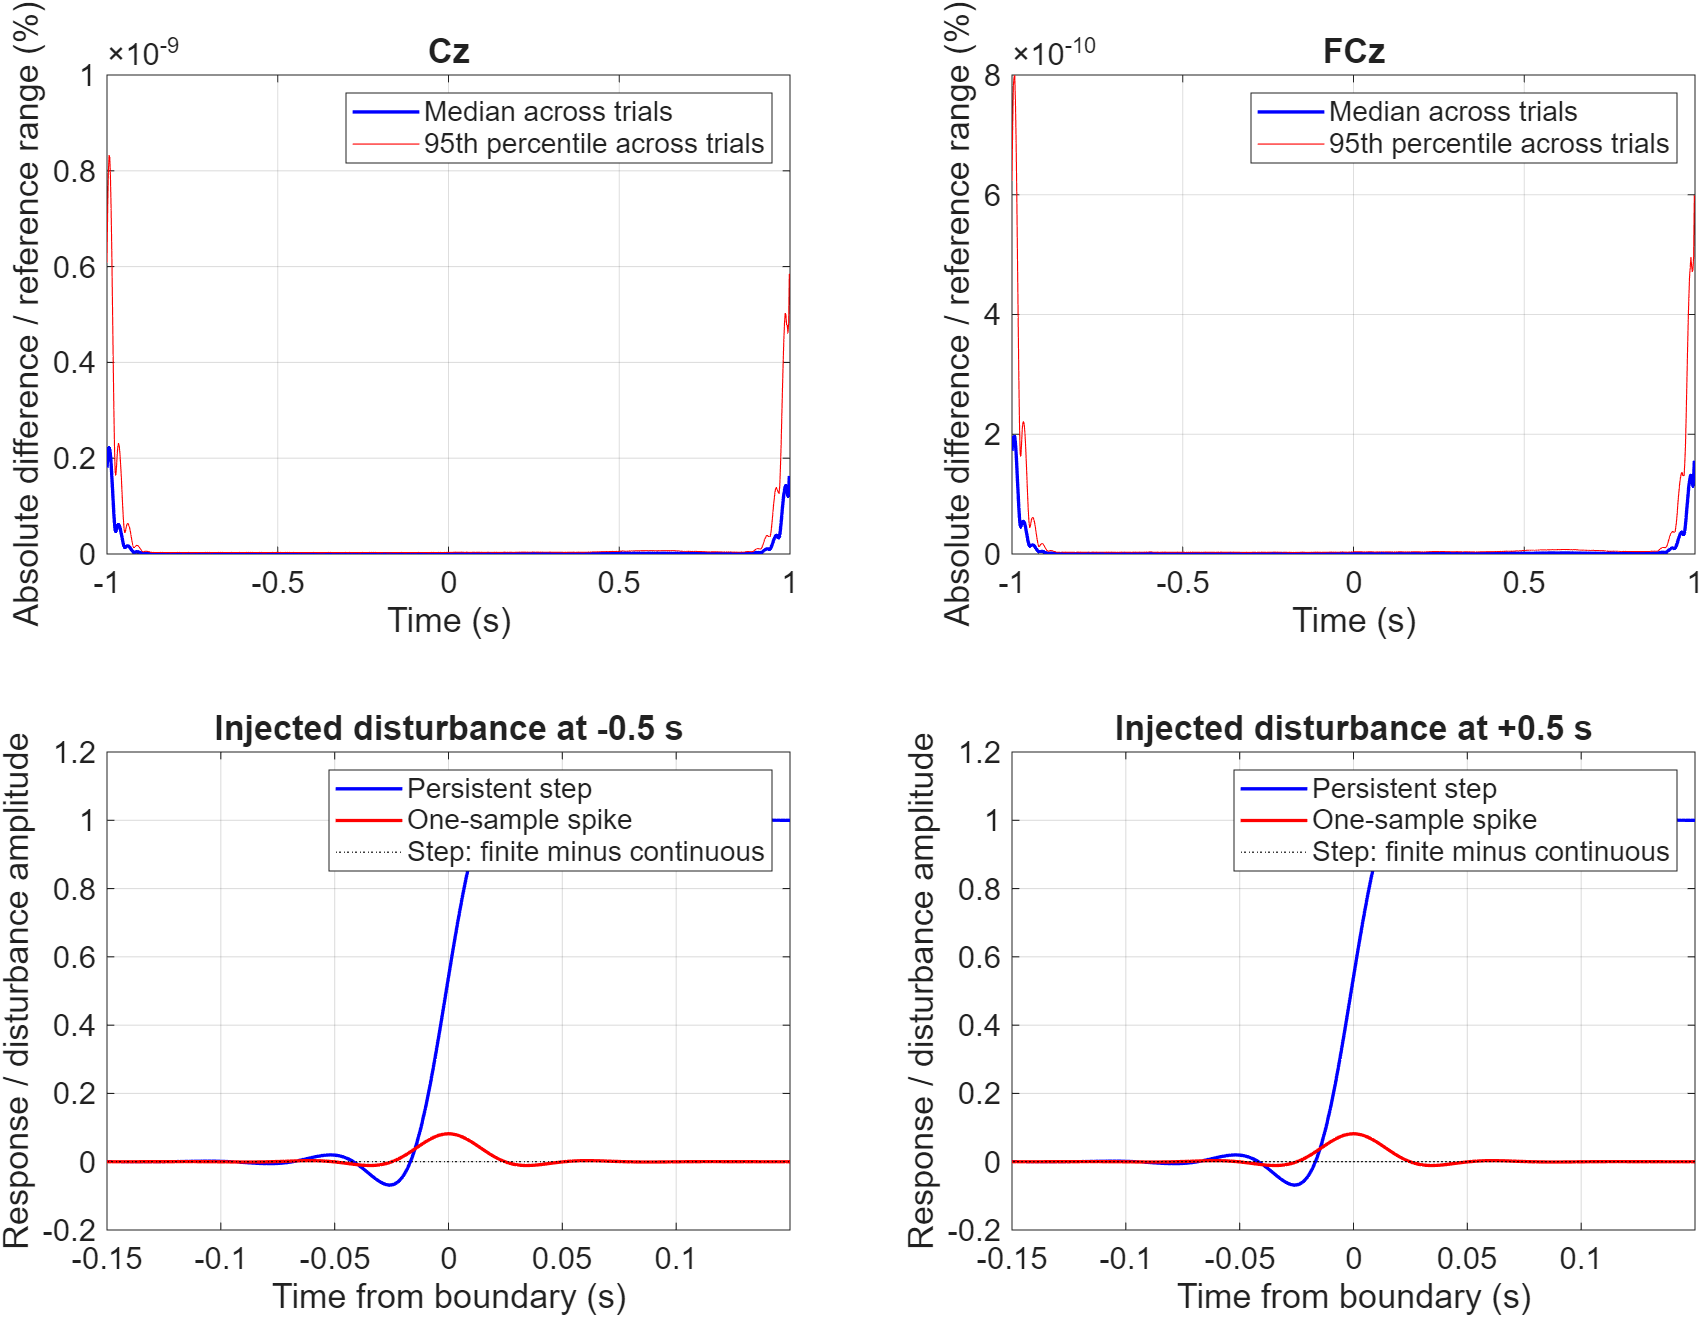
\includegraphics[width=\linewidth]{figures/filtering_effects.png}
\caption{\label{fig:filtering}Top: finite-segment versus continuous low-pass filtering, shown as absolute normalised difference envelopes across matched trials. Bottom: persistent-step and one-sample-spike responses normalised by injected amplitude. A smoothed persistent step still retains a level change; short-minus-long filtering isolates endpoint effects.}\end{figure}
\subsubsection{Synthetic boundary spreading}
Figure~\ref{fig:filtering} (bottom) shows close-ups around each injected boundary. A persistent unit level change becomes a smooth transition but retains its level difference; a one-sample spike becomes a broader, lower-amplitude response. The short-minus-long curve isolates segment-end effects. This explains why adjacent-sample attenuation alone is insufficient.
\subsubsection{Response-interval waveform differences}
Contrast 1: condition 3 minus the additional continuous sequential-filter reference (not condition 1). Contrast 2: split FORCe minus its control. Contrast 3: bandpass FORCe minus its control. Each entry is the median across trials of an absolute-residual statistic in 0.2--0.9~s. The control for contrast 2 is condition 3, and for contrast 3 it is condition 1. The first numeric column summarises within-trial median absolute residuals. The second normalises each trial by $S$ before taking the median. The final column summarises within-trial 95th-percentile absolute residuals divided by $S$; it is not a percentile pooled across samples or trials.
\begin{center}\small\begin{tabular}{rlrrr}\toprule
Contrast & Ch. & Median (\uv) & Median/$S$ (\%) & Trial $Q_{95}/S$ (\%) \\
\midrule
1 & Cz & $3.25\times10^{-13}$ & $1.21\times10^{-12}$ & $4.97\times10^{-12}$ \\
1 & FCz & $3.36\times10^{-13}$ & $1.19\times10^{-12}$ & $5.00\times10^{-12}$ \\
2 & Cz & 2.47350 & 9.502 & 49.343 \\
2 & FCz & 2.80303 & 9.968 & 51.860 \\
3 & Cz & 2.21061 & 8.298 & 44.863 \\
3 & FCz & 2.48240 & 8.813 & 47.376 \\
\bottomrule\end{tabular}\end{center}
Cleaning residuals contain intended removal as well as possible unwanted changes. The appendix shows condition-difference waveforms and extrema. Changes in the largest peak can reflect a different selected extremum, rather than latency movement of the same physiological component.
\subsubsection{Centring and reconstruction audit}
\begin{center}\small\begin{tabular}{llrrr}\toprule
Participant & Ch. & Windows & $|\mathrm{shift}|$ (\uv) & Max nonconstant RMS (\uv) \\
\midrule
mle01 & Cz & 135 & 0.601 & $<7.31\times10^{-8}$ \\
mle01 & FCz & 135 & 0.608 & $<8.44\times10^{-8}$ \\
spe30 & Cz & 126 & 0.838 & $<8.44\times10^{-8}$ \\
spe30 & FCz & 126 & 0.954 & $<1.34\times10^{-7}$ \\
\bottomrule\end{tabular}\end{center}
Median absolute shift is 0.734~\uv. The saved median nonconstant RMS is numerically zero, with an overall maximum of $1.33\times10^{-7}$~\uv. This estimate uses $\sqrt{\max(0,\mathrm{RMS}^2-\mathrm{shift}^2)}$; subtraction and clipping near floating-point precision can return zero. The table therefore reports upper bounds on the saved maximum nonconstant RMS, rather than six-decimal median zeros. Nonconstant RMS values at floating-point resolution are not evidence of mathematically exact zero. Reconstruction without rejection differs from the input mainly by a constant window-level shift. Different neighbouring shifts could contribute to joins, but their signed contribution to the final cleaned jumps is not quantified here. The audit therefore does not attribute all jumps to centring or justify restoring means without review.
\section{Discussion and limits}
\textbf{Boundary findings (Q1).} The exact split-filter control distinguishes cleaning effects from filtering implementation effects. All four conditions are needed for this attribution even though condition 3 is not a proposed final pipeline.


\textbf{Filtering findings (Q2).} Three-second extraction provides 0.5~s of additional context beyond each cropped endpoint, but leaves joins at $-0.5$ and $+0.5$~s inside the retained epoch. A low-pass attenuates sharp changes; it need not remove a sustained shift. The synthetic response describes known disturbances, not every real FORCe reconstruction effect.


\textbf{Interpretation and remaining limits.} Individual-trial distributions take priority over averages for the boundary question. Conversely, no-FORCe data are not neural ground truth, and a cleaning residual does not distinguish artifact from neural content. Visual smoothness, rarity, residual size and apparent peak changes must be interpreted together.
The practical result is a strong reduction in sharp boundary steps under the proposed processing, with negligible outer-endpoint filtering residuals in the tested no-FORCe control. Endpoint effects on FORCe-cleaned segments are not directly bounded by that control. However, median response-interval cleaning residuals remain about 9.5--10.0\% of the reference voltage range in the proposed condition. 

For example, spe30/pre/Cz has a positive maximum of 21.407~\uv\ in the bandpass no-FORCe reference versus 8.616~\uv\ with split-filter FORCe; its largest-absolute-peak time changes from 0.646 to 0.496~s. The split no-FORCe reference remains close to the bandpass reference (21.506~\uv, 0.644~s). This is a substantial waveform change, not proof of improved or damaged neural signals. The peak-time difference may reflect selection of a different extremum, particularly near the +0.5~s join. Those changes cannot be classified as artifact removal or neural distortion from this pilot alone. 

The pilot does not retune FORCe, benchmark artifact removal, establish classifier performance, or support population-level inference. Retaining FORCe should depend on useful artifact handling without unacceptable response changes. Proceeding without it remains an option.
\begin{thebibliography}{9}
\bibitem{daly} Daly I, Scherer R, Billinger M, M\"uller-Putz G. FORCe: Fully Online and Automated Artifact Removal for Brain-Computer Interfacing. \emph{IEEE Transactions on Neural Systems and Rehabilitation Engineering}. 2015;23(5):725--736. \href{https://doi.org/10.1109/TNSRE.2014.2346621}{doi:10.1109/TNSRE.2014.2346621}.
\bibitem{graz} Amaunam I, Sultana M, Rodriguez-Herreros B, Tadi T, Leeb R, Perdikis S. EEG correlates of error-related activity during ballistic computer mouse movements. Graz BCI Conference, 2024. Supplied manuscript.
\bibitem{widmann} Widmann A, Schr\"oger E. Filter Effects and Filter Artifacts in the Analysis of Electrophysiological Data. \emph{Frontiers in Psychology}. 2012;3:233. \href{https://doi.org/10.3389/fpsyg.2012.00233}{doi:10.3389/fpsyg.2012.00233}.
\end{thebibliography}
\clearpage\appendix\section{Participant-specific boundary statistics}
\textit{Condition key: 1 = bandpass/no FORCe; 2 = bandpass/FORCe; 3 = split/no FORCe; 4 = split/FORCe.}

\small\begin{longtable}{llcrrrr}\toprule Participant & Ch. & Join & ID & Median (\uv) & $J/S$ (\%) & \shortstack{Trials $\geq Q_{99}$\\(\%)}\\\midrule\endhead
mle01 & Cz & -0.5 & 1 & 0.330 & 1.43 & 1.1 \\
mle01 & Cz & -0.5 & 2 & 1.426 & 5.87 & 39.5 \\
mle01 & Cz & -0.5 & 3 & 0.289 & 1.24 & 1.8 \\
mle01 & Cz & -0.5 & 4 & 0.328 & 1.42 & 1.1 \\
mle01 & Cz & +0.5 & 1 & 0.370 & 1.53 & 1.4 \\
mle01 & Cz & +0.5 & 2 & 2.816 & 11.93 & 60.6 \\
mle01 & Cz & +0.5 & 3 & 0.368 & 1.63 & 3.5 \\
mle01 & Cz & +0.5 & 4 & 0.369 & 1.51 & 1.4 \\
mle01 & FCz & -0.5 & 1 & 0.328 & 1.37 & 1.2 \\
mle01 & FCz & -0.5 & 2 & 1.421 & 5.90 & 40.1 \\
mle01 & FCz & -0.5 & 3 & 0.285 & 1.19 & 2.0 \\
mle01 & FCz & -0.5 & 4 & 0.325 & 1.36 & 1.2 \\
mle01 & FCz & +0.5 & 1 & 0.383 & 1.50 & 1.1 \\
mle01 & FCz & +0.5 & 2 & 3.049 & 12.43 & 62.7 \\
mle01 & FCz & +0.5 & 3 & 0.383 & 1.59 & 3.8 \\
mle01 & FCz & +0.5 & 4 & 0.385 & 1.51 & 1.1 \\
spe30 & Cz & -0.5 & 1 & 0.330 & 1.17 & 0.1 \\
spe30 & Cz & -0.5 & 2 & 1.686 & 5.81 & 44.7 \\
spe30 & Cz & -0.5 & 3 & 0.320 & 1.13 & 1.1 \\
spe30 & Cz & -0.5 & 4 & 0.327 & 1.15 & 0.1 \\
spe30 & Cz & +0.5 & 1 & 0.447 & 1.59 & 2.7 \\
spe30 & Cz & +0.5 & 2 & 4.730 & 16.83 & 72.2 \\
spe30 & Cz & +0.5 & 3 & 0.509 & 1.82 & 7.7 \\
spe30 & Cz & +0.5 & 4 & 0.452 & 1.57 & 2.9 \\
spe30 & FCz & -0.5 & 1 & 0.344 & 1.12 & 0.3 \\
spe30 & FCz & -0.5 & 2 & 1.928 & 6.24 & 46.8 \\
spe30 & FCz & -0.5 & 3 & 0.337 & 1.07 & 1.0 \\
spe30 & FCz & -0.5 & 4 & 0.344 & 1.11 & 0.2 \\
spe30 & FCz & +0.5 & 1 & 0.474 & 1.55 & 3.1 \\
spe30 & FCz & +0.5 & 2 & 5.495 & 18.03 & 73.8 \\
spe30 & FCz & +0.5 & 3 & 0.550 & 1.83 & 9.4 \\
spe30 & FCz & +0.5 & 4 & 0.476 & 1.54 & 3.1 \\
\bottomrule\end{longtable}\normalsize
\section{Onset and maximum-channel supporting summaries}
\textit{Condition key: 1 = bandpass/no FORCe; 2 = bandpass/FORCe; 3 = split/no FORCe; 4 = split/FORCe.}

Movement onset is not a join in these conditions. Maximum-channel measurements select each trial's largest raw step, then use that channel's ordinary-change distribution. They can select different channels across conditions.
\begin{center}\small\begin{tabular}{lcrrrrr}\toprule
Channel & Time & ID & Median (\uv) & $Q_{95}$ (\uv) & Max (\uv) & \shortstack{Trials $\geq Q_{99}$\\(\%)} \\
\midrule
Cz & +0.0 & 1 & 0.350 & 1.276 & 2.812 & 0.7 \\
Cz & +0.0 & 2 & 0.363 & 1.316 & 3.273 & 1.1 \\
Cz & +0.0 & 4 & 0.282 & 0.990 & 2.510 & 1.4 \\
Cz & +0.0 & 3 & 0.344 & 1.262 & 2.806 & 0.7 \\
FCz & +0.0 & 1 & 0.356 & 1.283 & 2.837 & 0.7 \\
FCz & +0.0 & 2 & 0.377 & 1.340 & 3.304 & 1.1 \\
FCz & +0.0 & 4 & 0.289 & 1.006 & 2.575 & 1.3 \\
FCz & +0.0 & 3 & 0.352 & 1.279 & 2.833 & 0.7 \\
Max-eight & -0.5 & 1 & 0.556 & 1.337 & 6.984 & 1.4 \\
Max-eight & -0.5 & 2 & 2.242 & 11.481 & 83.707 & 57.7 \\
Max-eight & -0.5 & 4 & 0.511 & 1.189 & 4.678 & 2.9 \\
Max-eight & -0.5 & 3 & 0.550 & 1.329 & 6.958 & 1.3 \\
Max-eight & +0.0 & 1 & 0.567 & 1.492 & 2.837 & 1.6 \\
Max-eight & +0.0 & 2 & 0.646 & 1.527 & 3.306 & 2.9 \\
Max-eight & +0.0 & 4 & 0.483 & 1.198 & 2.575 & 2.8 \\
Max-eight & +0.0 & 3 & 0.564 & 1.480 & 2.833 & 1.6 \\
Max-eight & +0.5 & 1 & 0.642 & 1.667 & 3.733 & 3.9 \\
Max-eight & +0.5 & 2 & 5.262 & 19.637 & 39.407 & 81.8 \\
Max-eight & +0.5 & 4 & 0.655 & 1.658 & 3.118 & 11.0 \\
Max-eight & +0.5 & 3 & 0.637 & 1.647 & 3.752 & 3.8 \\
\bottomrule\end{tabular}\end{center}
\clearpage\section{Condition-difference waveforms}
\textit{Condition key: 1 = bandpass/no FORCe; 2 = bandpass/FORCe; 3 = split/no FORCe; 4 = split/FORCe.}

\begin{figure}[htbp]\centering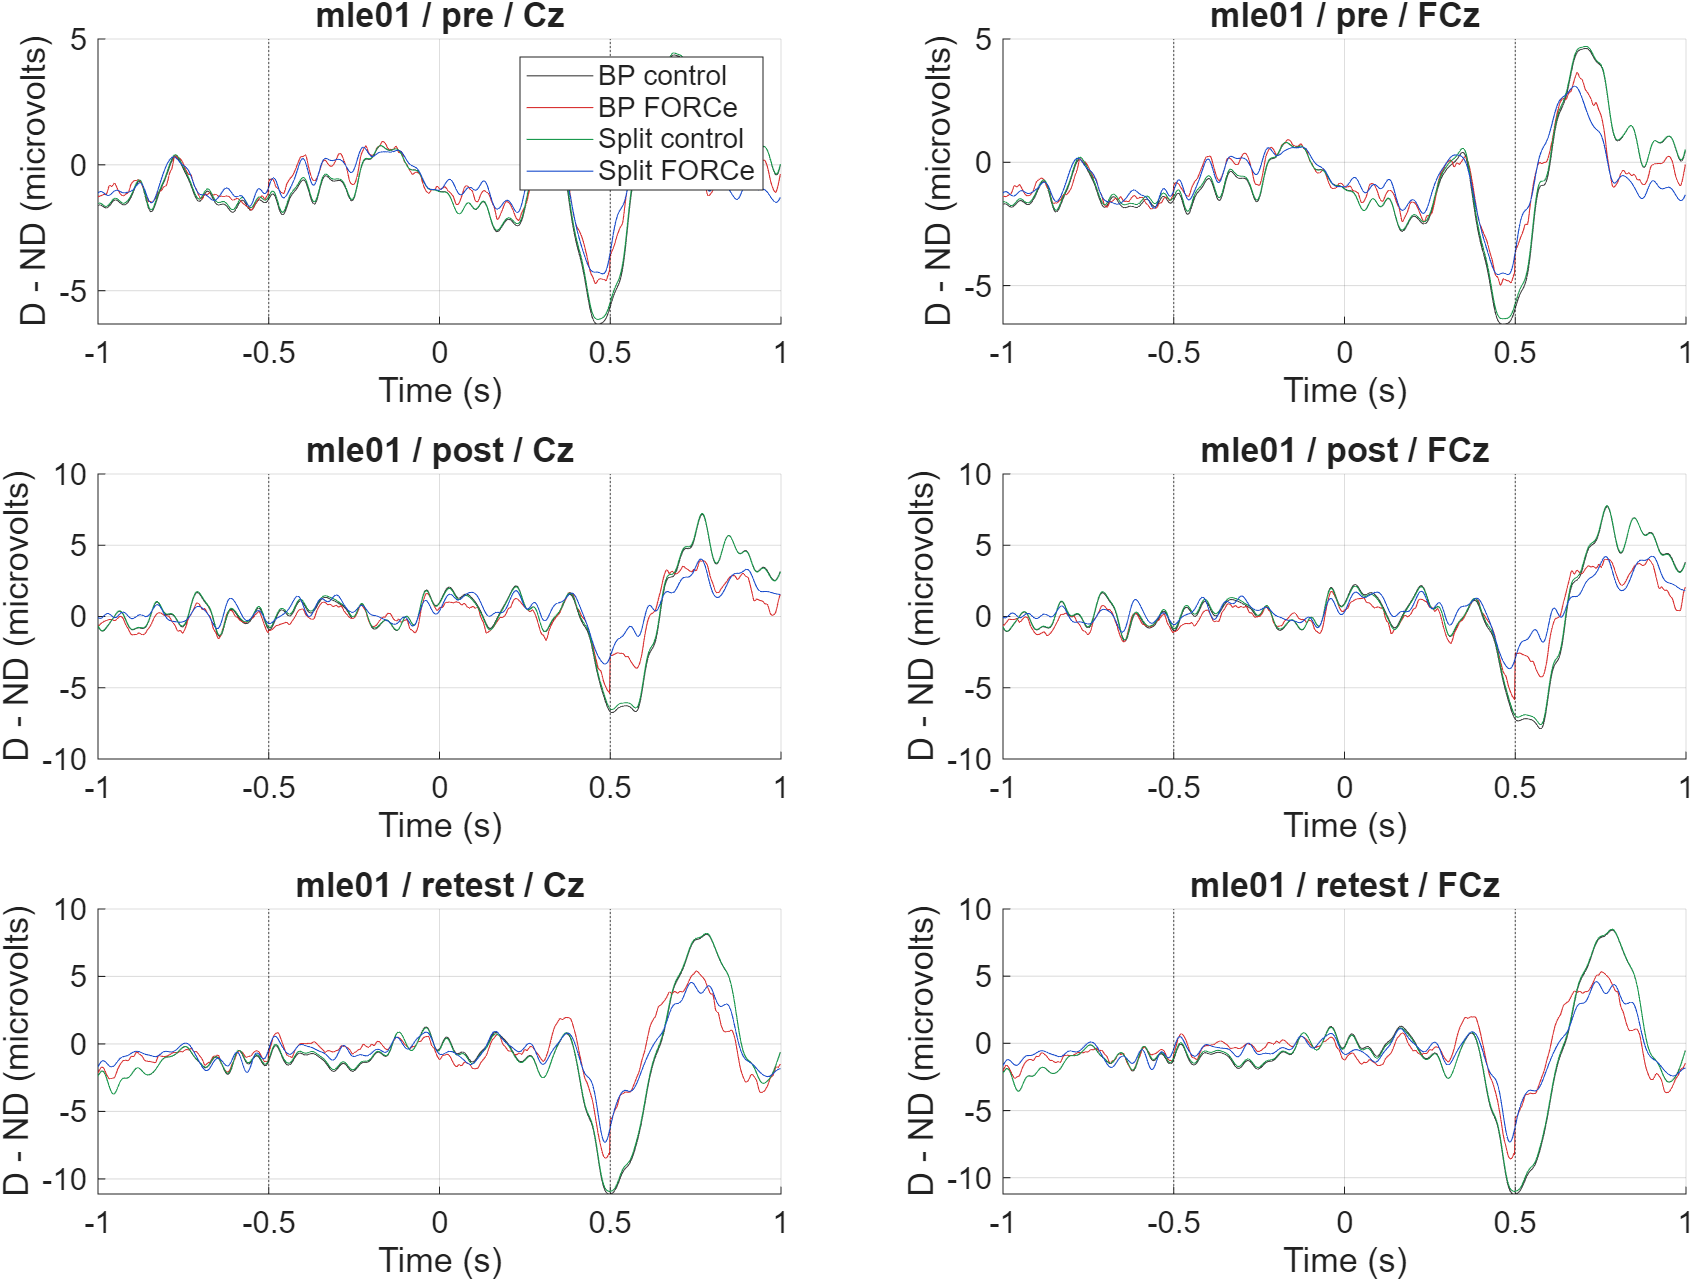
\includegraphics[width=\linewidth]{figures/erp_differences_1.png}
\caption{Matched displaced-minus-non-displaced waveforms for mle01, by session and channel. Joins are at -0.5 and +0.5 s.}\end{figure}
\begin{figure}[htbp]\centering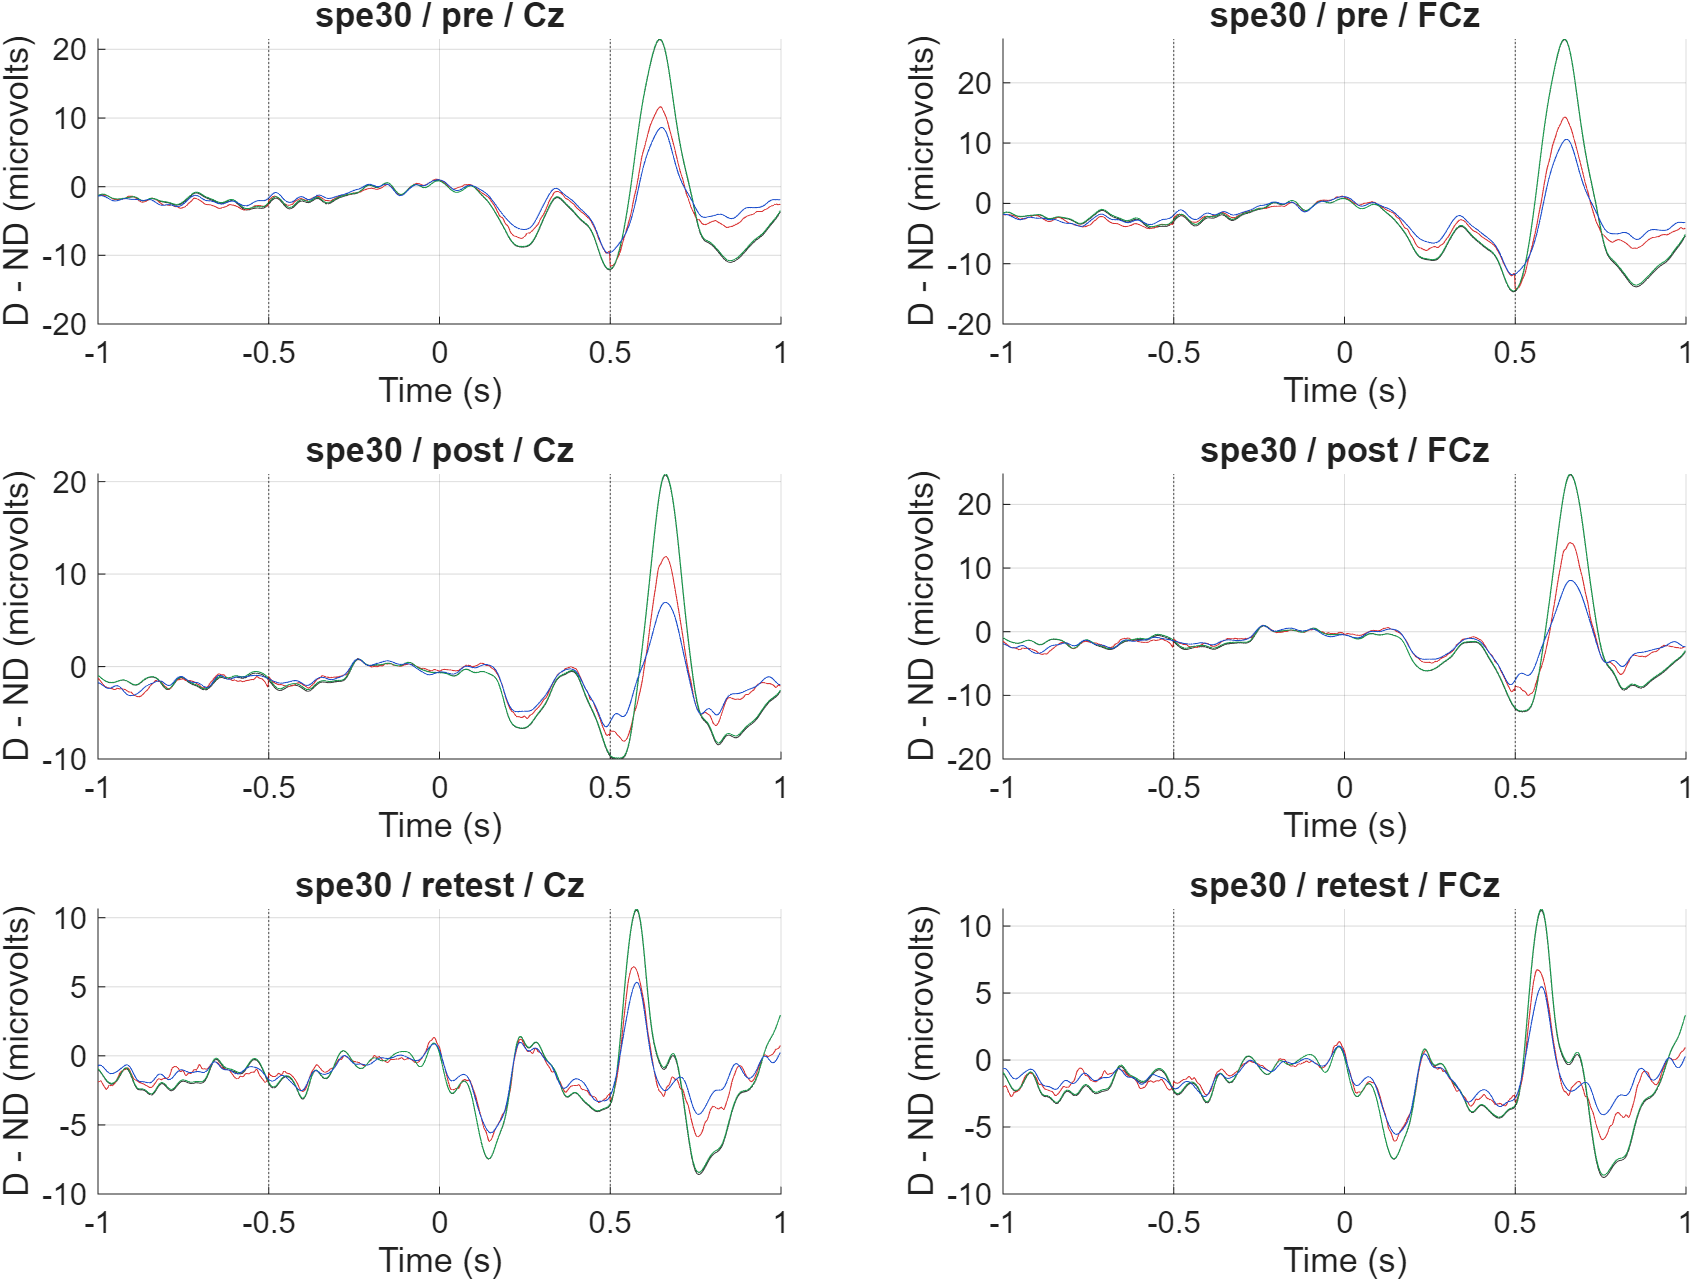
\includegraphics[width=\linewidth]{figures/erp_differences_2.png}
\caption{Matched displaced-minus-non-displaced waveforms for spe30, by session and channel. Joins are at -0.5 and +0.5 s.}\end{figure}
\begin{figure}[htbp]\centering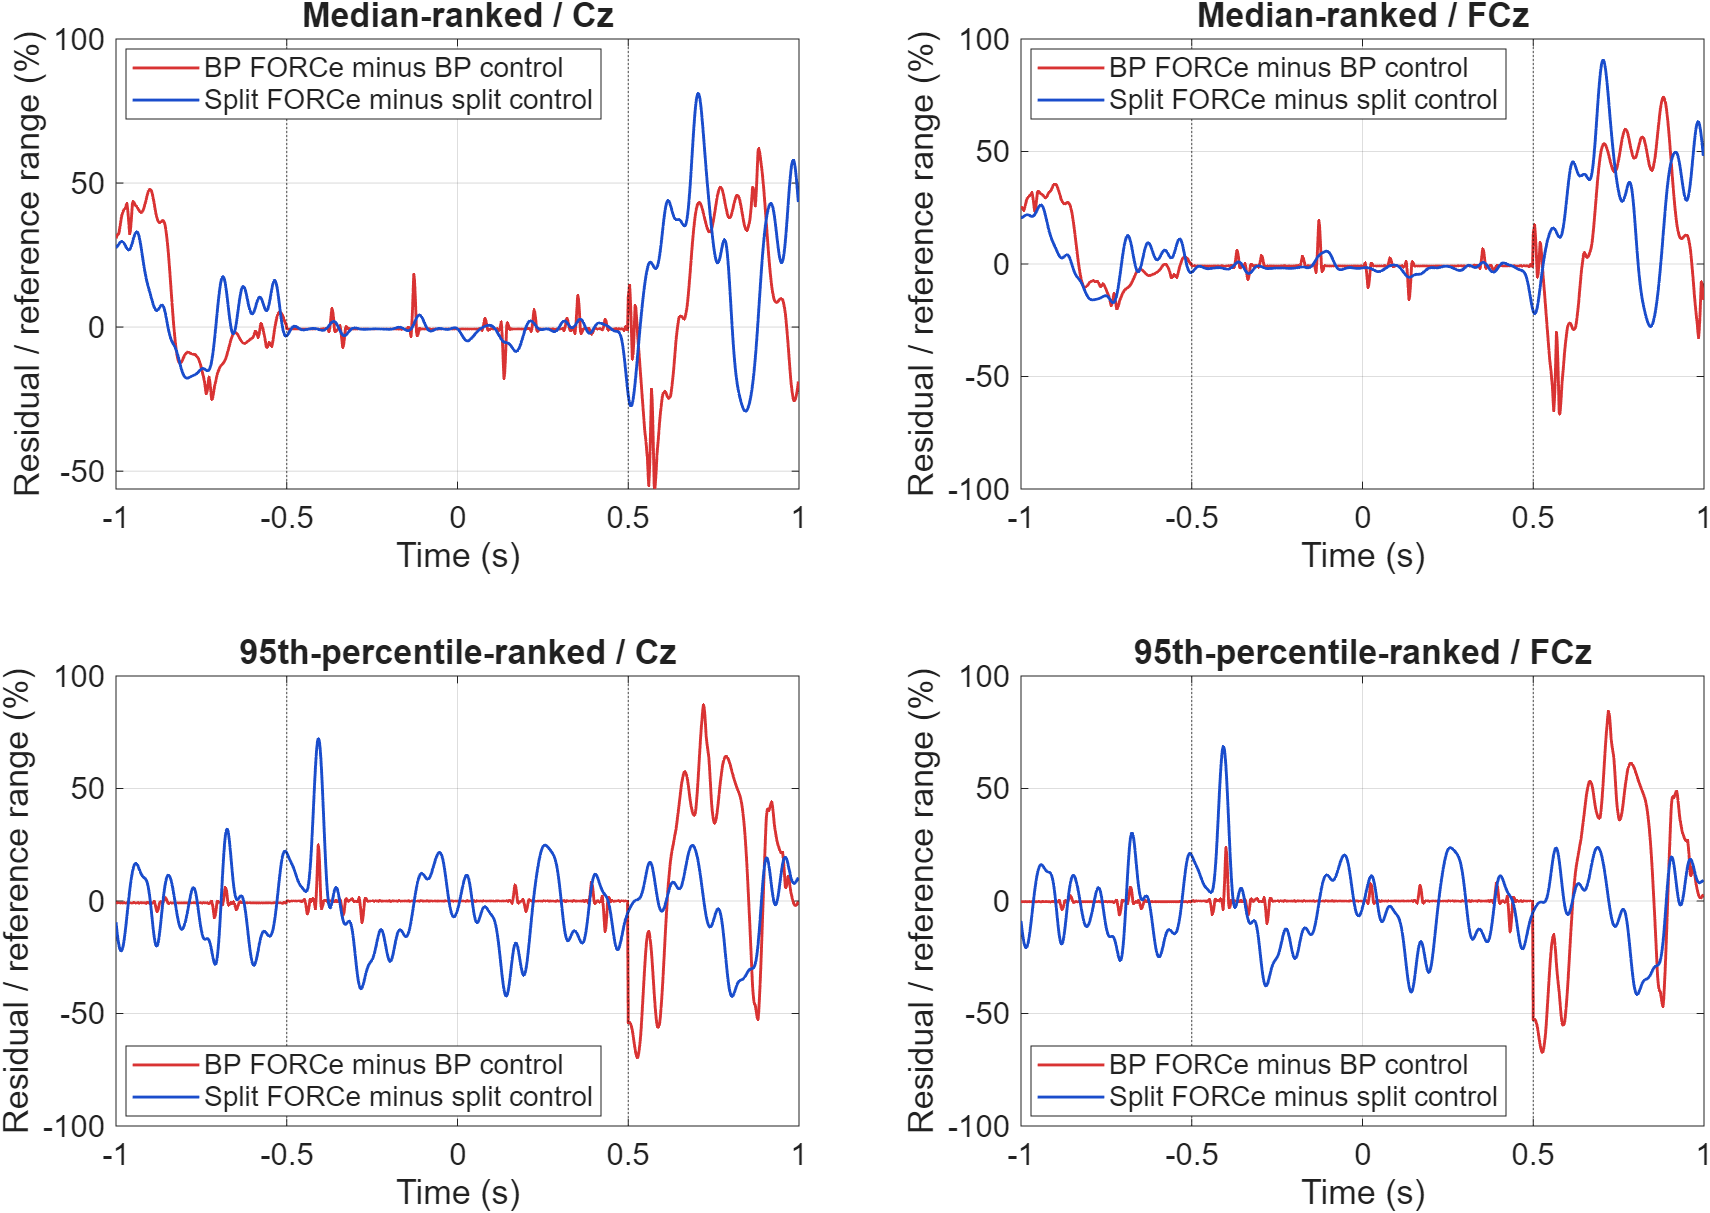
\includegraphics[width=\linewidth]{figures/actual_cleaning_residuals.png}
\caption{Actual cleaning residuals for the same representative trials, in Cz and FCz. Both curves use the common condition-1 voltage scale. These differences include artifact removal and are not neural-error estimates.}\end{figure}
\clearpage\section{ERP extrema and peak-time descriptions}
\textit{Condition key: 1 = bandpass/no FORCe; 2 = bandpass/FORCe; 3 = split/no FORCe; 4 = split/FORCe.}
\small\begin{longtable}{lllrrrr}\toprule Participant & Session & Ch. & ID & Min (\uv) & Max (\uv) & Peak time (s)\\\midrule\endhead
mle01 & pre & Cz & 1 & -6.324 & 4.365 & 0.464 \\
mle01 & pre & Cz & 2 & -4.716 & 3.698 & 0.456 \\
mle01 & pre & Cz & 4 & -4.330 & 3.147 & 0.478 \\
mle01 & pre & Cz & 3 & -6.137 & 4.445 & 0.464 \\
mle01 & pre & FCz & 1 & -6.559 & 4.616 & 0.464 \\
mle01 & pre & FCz & 2 & -4.984 & 3.633 & 0.456 \\
mle01 & pre & FCz & 4 & -4.551 & 3.089 & 0.478 \\
mle01 & pre & FCz & 3 & -6.348 & 4.699 & 0.462 \\
mle01 & post & Cz & 1 & -6.746 & 7.167 & 0.770 \\
mle01 & post & Cz & 2 & -5.377 & 3.919 & 0.498 \\
mle01 & post & Cz & 4 & -3.334 & 4.027 & 0.766 \\
mle01 & post & Cz & 3 & -6.531 & 7.232 & 0.770 \\
mle01 & post & FCz & 1 & -7.878 & 7.694 & 0.574 \\
mle01 & post & FCz & 2 & -5.840 & 4.026 & 0.498 \\
mle01 & post & FCz & 4 & -3.659 & 4.214 & 0.898 \\
mle01 & post & FCz & 3 & -7.586 & 7.773 & 0.768 \\
mle01 & retest & Cz & 1 & -11.119 & 8.129 & 0.498 \\
mle01 & retest & Cz & 2 & -8.459 & 5.411 & 0.488 \\
mle01 & retest & Cz & 4 & -7.284 & 4.562 & 0.484 \\
mle01 & retest & Cz & 3 & -10.921 & 8.201 & 0.498 \\
mle01 & retest & FCz & 1 & -11.215 & 8.431 & 0.498 \\
mle01 & retest & FCz & 2 & -8.612 & 5.333 & 0.488 \\
mle01 & retest & FCz & 4 & -7.348 & 4.592 & 0.484 \\
mle01 & retest & FCz & 3 & -11.016 & 8.501 & 0.498 \\
spe30 & pre & Cz & 1 & -12.104 & 21.407 & 0.646 \\
spe30 & pre & Cz & 2 & -11.545 & 11.641 & 0.648 \\
spe30 & pre & Cz & 4 & -9.668 & 8.616 & 0.496 \\
spe30 & pre & Cz & 3 & -12.007 & 21.506 & 0.644 \\
spe30 & pre & FCz & 1 & -14.643 & 27.149 & 0.644 \\
spe30 & pre & FCz & 2 & -14.220 & 14.290 & 0.646 \\
spe30 & pre & FCz & 4 & -11.845 & 10.636 & 0.492 \\
spe30 & pre & FCz & 3 & -14.518 & 27.261 & 0.644 \\
spe30 & post & Cz & 1 & -9.988 & 20.703 & 0.662 \\
spe30 & post & Cz & 2 & -8.065 & 11.882 & 0.662 \\
spe30 & post & Cz & 4 & -6.511 & 6.950 & 0.662 \\
spe30 & post & Cz & 3 & -9.887 & 20.824 & 0.662 \\
spe30 & post & FCz & 1 & -12.577 & 24.655 & 0.662 \\
spe30 & post & FCz & 2 & -9.999 & 14.002 & 0.660 \\
spe30 & post & FCz & 4 & -8.319 & 8.076 & 0.486 \\
spe30 & post & FCz & 3 & -12.456 & 24.790 & 0.662 \\
spe30 & retest & Cz & 1 & -8.588 & 10.533 & 0.576 \\
spe30 & retest & Cz & 2 & -5.866 & 6.441 & 0.568 \\
spe30 & retest & Cz & 4 & -4.232 & 5.316 & 0.578 \\
spe30 & retest & Cz & 3 & -8.432 & 10.629 & 0.576 \\
spe30 & retest & FCz & 1 & -8.763 & 11.157 & 0.576 \\
spe30 & retest & FCz & 2 & -5.937 & 6.734 & 0.566 \\
spe30 & retest & FCz & 4 & -4.085 & 5.463 & 0.578 \\
spe30 & retest & FCz & 3 & -8.589 & 11.270 & 0.576 \\
\bottomrule\end{longtable}\normalsize
\end{document}
